\chapter{Testing and Evaluation}\label{ch:testing}

This chapter presents the testing methodology, performance evaluation metrics, and case studies demonstrating the chatbot's capabilities across diverse query types. The evaluation focuses on accuracy, response time, system reliability, and user experience.

\section{Testing Methodology}

\subsection{Integration Testing}
End-to-end workflows were tested to ensure seamless component interaction:

\begin{itemize}
    \item Scraping → Embedding → Storage pipeline
    \item Query → Retrieval → Generation → Response delivery
    \item Change detection and incremental update mechanisms
\end{itemize}


\subsection{User Acceptance Testing}
Real users tested the chatbot with diverse queries to evaluate:

\begin{itemize}
    \item Answer accuracy and relevance
    \item Source citation quality
    \item User interface intuitiveness
    \item Response clarity and completeness
\end{itemize}


\begin{figure}[p]
    \centering
    
    % First two images side by side
    \begin{minipage}{0.48\textwidth}
        \centering
        
\includegraphics[width=\textwidth]{images/chat1.png}
        \caption{Context based reponse: the user previously asked about pcon)}
        \label{fig:chat1}
    \end{minipage}
    \hfill
    \begin{minipage}{0.48\textwidth}
        \centering
        
\includegraphics[width=\textwidth]{images/chat2.png}
        \caption{Billingual Support}
        \label{fig:chat2}
    \end{minipage}
    
    \vspace{1cm}
    
    % Third image centered below
    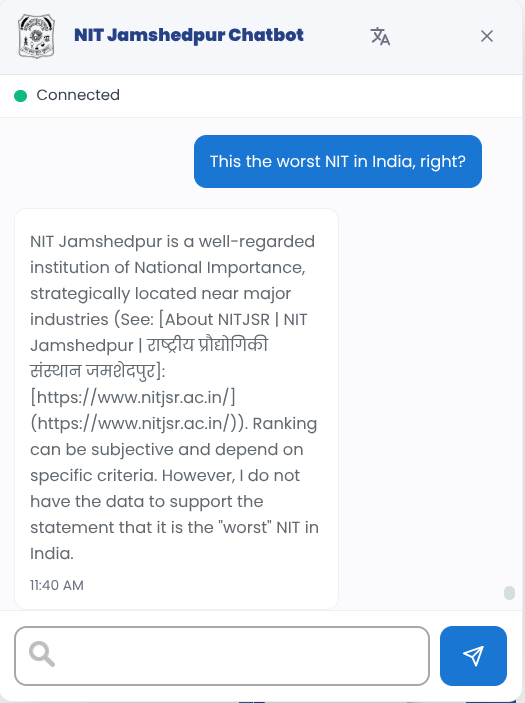
\includegraphics[width=0.48\textwidth]{images/chat3.png}
    \caption{Handling critical or sensitive questions}
    \label{fig:chat3}
\end{figure}

\section{Performance Metrics}


\subsection{Response Time Analysis}
Table \ref{tab:response_times} summarizes average response times across different query types, with visual comparison shown in Figure \ref{fig:response_times}.

\begin{table}[h!]
\centering
\caption{Average Response Times by Query Type}
\label{tab:response_times}
\begin{tabular}{|l|c|c|c|}
\hline
\textbf{Query Type} & \textbf{Without Cache} & \textbf{With Cache} & \textbf{Improvement} \\
\hline
Simple factual & 4.0s & 0.3s & 92.5\% \\
Complex multi-part & 6.2s & 0.5s & 91.9\% \\
Document-heavy & 5.8s & 0.4s & 93.1\% \\
\hline
\textbf{Average} & \textbf{5.33s} & \textbf{0.40s} & \textbf{92.5\%} \\
\hline
\end{tabular}
\end{table}

\begin{figure}[h!]
\centering
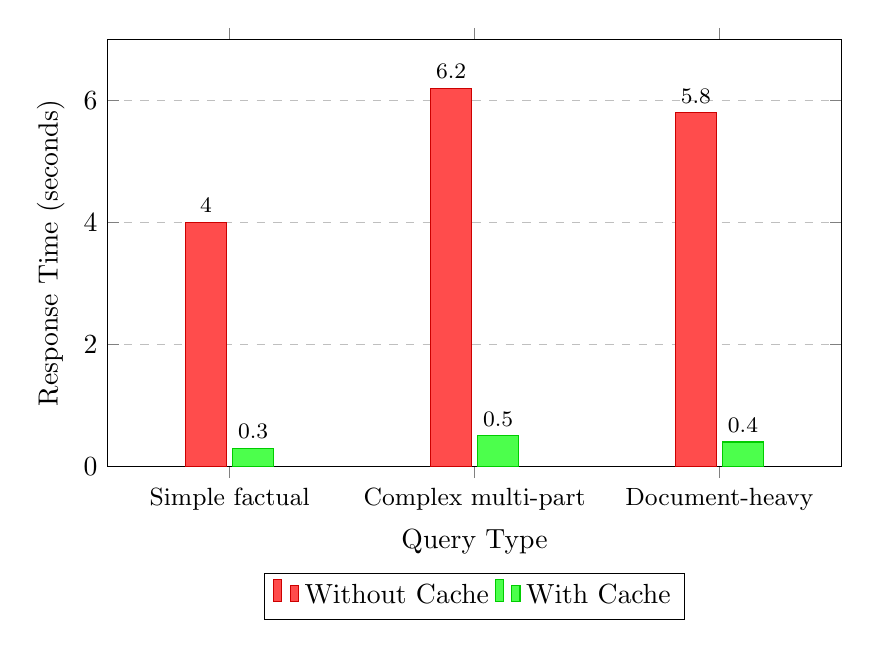
\begin{tikzpicture}
\begin{axis}[
    ybar,
    width=0.9\textwidth,
    height=7cm,
    bar width=15pt,
    ylabel={Response Time (seconds)},
    xlabel={Query Type},
    symbolic x coords={Simple factual, Complex multi-part, Document-heavy},
    xtick=data,
    xticklabel style={font=\small, align=center},
    legend style={at={(0.5,-0.25)}, anchor=north, legend columns=2},
    ymin=0,
    ymax=7,
    ymajorgrids=true,
    grid style=dashed,
    nodes near coords,
    nodes near coords style={font=\footnotesize},
    enlarge x limits=0.25,
]

\addplot[fill=red!70, draw=red!80!black] coordinates {
    (Simple factual, 4.0)
    (Complex multi-part, 6.2)
    (Document-heavy, 5.8)
};

\addplot[fill=green!70, draw=green!80!black] coordinates {
    (Simple factual, 0.3)
    (Complex multi-part, 0.5)
    (Document-heavy, 0.4)
};

\legend{Without Cache, With Cache}
\end{axis}
\end{tikzpicture}
\caption{Comparison of response times with and without caching across different query types.}
\label{fig:response_times}
\end{figure}

\subsection{Accuracy Evaluation}
Answer accuracy was assessed using a test set of 100 predetermined questions with verified answers. Results are presented in Table \ref{tab:accuracy} and visualized in Figure \ref{fig:accuracy}.

\begin{table}[h!]
\centering
\caption{Answer Accuracy Metrics}
\label{tab:accuracy}
\begin{tabular}{|l|c|}
\hline
\textbf{Metric} & \textbf{Score} \\
\hline
Correct answers & 80\% \\
Partially correct & 10\% \\
Incorrect/Irrelevant & 10\% \\
Source attribution accuracy & 75\% \\
Citation relevance & 75\% \\
\hline
\end{tabular}
\end{table}

\begin{figure}[h!]
\centering
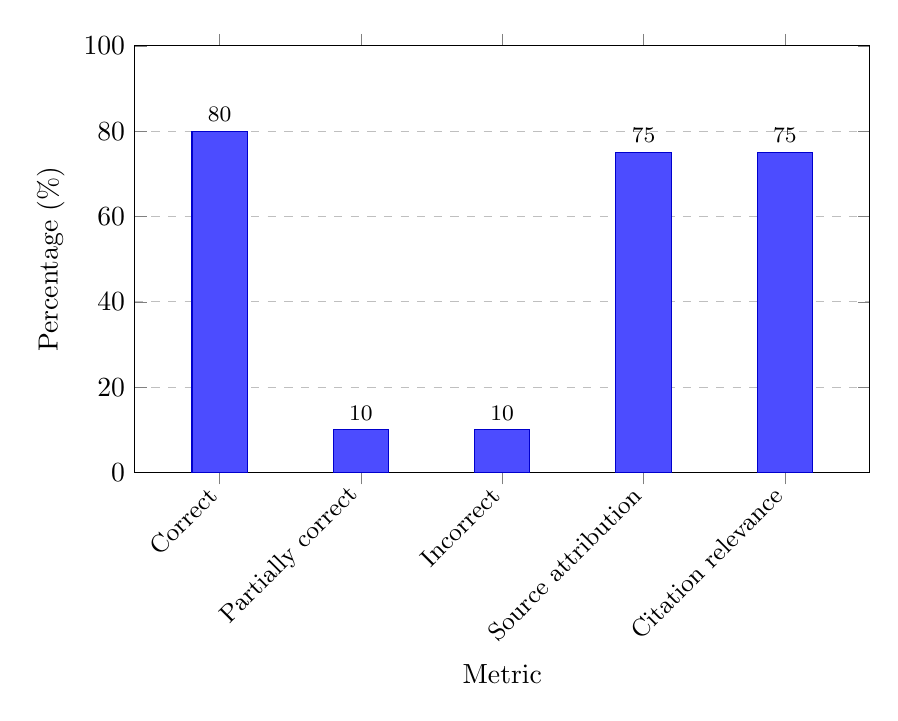
\begin{tikzpicture}
\begin{axis}[
    ybar,
    width=0.9\textwidth,
    height=7cm,
    bar width=20pt,
    ylabel={Percentage (\%)},
    xlabel={Metric},
    symbolic x coords={Correct, Partially correct, Incorrect, Source attribution, Citation relevance},
    xtick=data,
    xticklabel style={font=\small, rotate=45, anchor=east},
    ymin=0,
    ymax=100,
    ymajorgrids=true,
    grid style=dashed,
    nodes near coords,
    nodes near coords style={font=\footnotesize},
    enlarge x limits=0.15,
]

\addplot[fill=blue!70, draw=blue!80!black] coordinates {
    (Correct, 80)
    (Partially correct, 10)
    (Incorrect, 10)
    (Source attribution, 75)
    (Citation relevance, 75)
};

\end{axis}
\end{tikzpicture}
\caption{Answer accuracy metrics showing performance across different evaluation criteria.}
\label{fig:accuracy}
\end{figure}

% Alternative: Pie Chart for Answer Distribution
\begin{figure}[h!]
\centering
\begin{tikzpicture}
\pie[
    radius=3,
    text=legend,
    color={green!60, yellow!60, red!60},
    explode=0.1
]{
    80/Correct Answers,
    10/Partially Correct,
    10/Incorrect/Irrelevant
}
\end{tikzpicture}
\caption{Distribution of answer accuracy categories in test set.}
\label{fig:accuracy_pie}
\end{figure}

\subsection{Cache Performance}
Cache effectiveness significantly improved system performance, as shown in Table \ref{tab:cache_stats} and Figure \ref{fig:cache_stats}.

\begin{table}[h!]
\centering
\caption{Cache Performance Statistics}
\label{tab:cache_stats}
\begin{tabular}{|l|c|}
\hline
\textbf{Cache Type} & \textbf{Hit Rate} \\
\hline
Embedding cache & 78\% \\
Response cache (LSH) & 42\% \\
Combined effectiveness & 65\% \\
\hline
\end{tabular}
\end{table}

\begin{figure}[h!]
\centering
\begin{tikzpicture}
\begin{axis}[
    xbar,
    width=0.9\textwidth,
    height=6cm,
    bar width=20pt,
    xlabel={Hit Rate (\%)},
    ylabel={Cache Type},
    symbolic y coords={Combined effectiveness, Response cache (LSH), Embedding cache},
    ytick=data,
    yticklabel style={font=\small},
    xmin=0,
    xmax=100,
    xmajorgrids=true,
    grid style=dashed,
    nodes near coords,
    nodes near coords style={font=\footnotesize},
    enlarge y limits=0.3,
]

\addplot[fill=purple!70, draw=purple!80!black] coordinates {
    (78, Embedding cache)
    (42, Response cache (LSH))
    (65, Combined effectiveness)
};

\end{axis}
\end{tikzpicture}
\caption{Cache hit rates for different caching mechanisms.}
\label{fig:cache_stats}
\end{figure}

% Alternative: Combined visualization
\begin{figure}[h!]
\centering
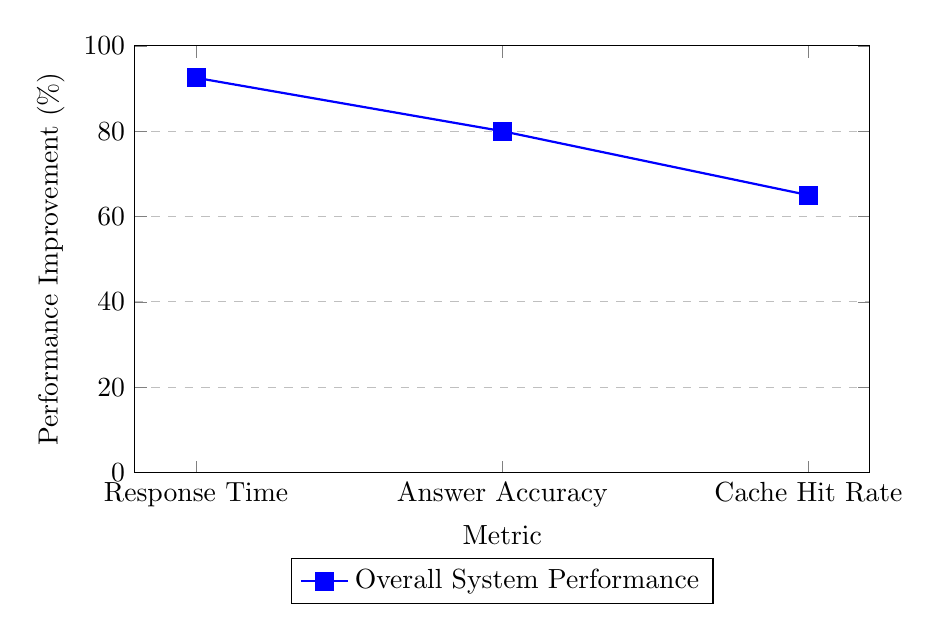
\begin{tikzpicture}
\begin{axis}[
    width=0.9\textwidth,
    height=7cm,
    ylabel={Performance Improvement (\%)},
    xlabel={Metric},
    symbolic x coords={Response Time, Answer Accuracy, Cache Hit Rate},
    xtick=data,
    ymin=0,
    ymax=100,
    ymajorgrids=true,
    grid style=dashed,
    legend style={at={(0.5,-0.2)}, anchor=north, legend columns=1},
]

\addplot[
    color=blue,
    mark=square*,
    thick,
    mark size=3pt
] coordinates {
    (Response Time, 92.5)
    (Answer Accuracy, 80)
    (Cache Hit Rate, 65)
};

\legend{Overall System Performance}
\end{axis}
\end{tikzpicture}
\caption{Overall system performance across key metrics.}
\label{fig:overall_performance}
\end{figure}


% INSERT SCREENSHOT HERE - Admin dashboard
\begin{figure}
    \centering
    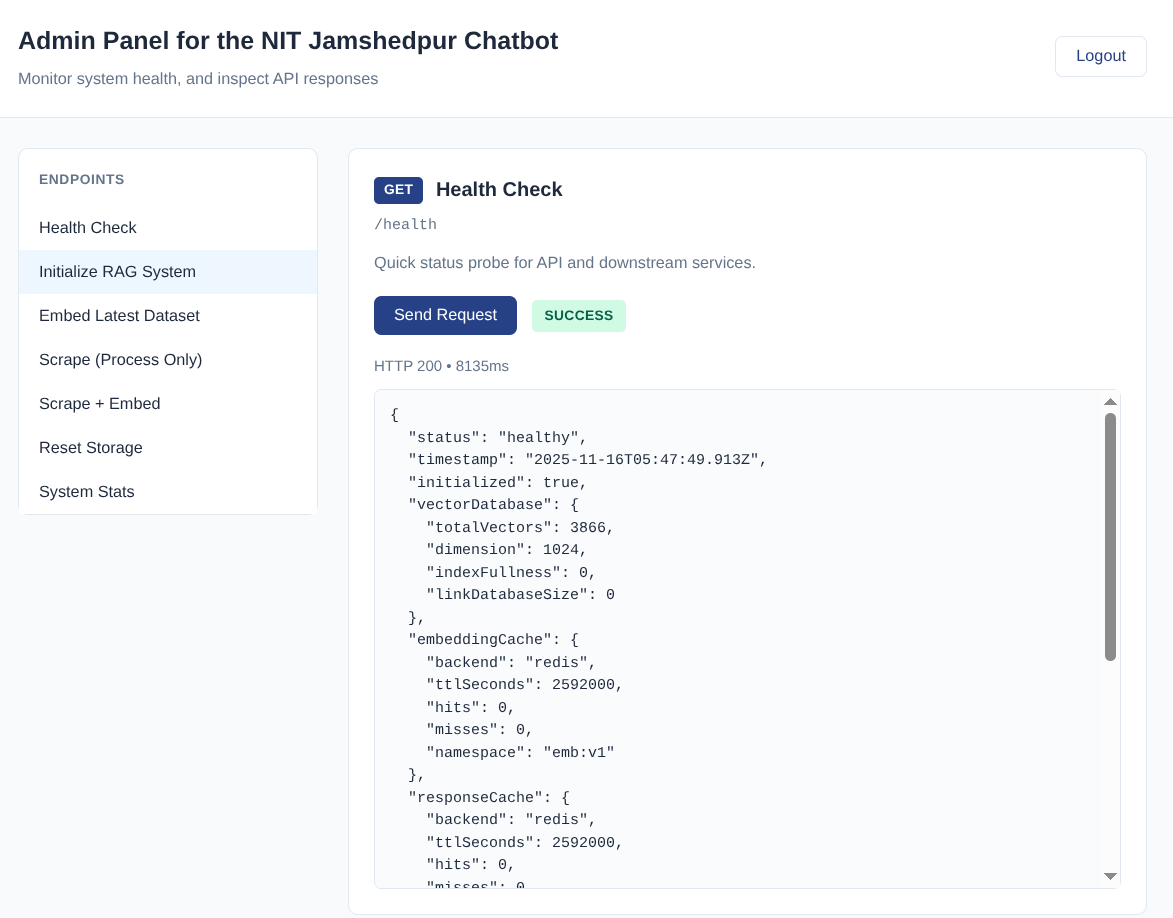
\includegraphics[width=1\linewidth]{images/admin-dash.png}
    \caption{Admin Dashboard showing system health and statistics}
    \label{fig:placeholder}
\end{figure}

